\documentclass[12pt]{article}
 
\usepackage[margin=.85in]{geometry} 
\usepackage{amsmath,amsthm,amssymb}
\usepackage{units}
\usepackage{bm}
\usepackage{enumitem}
\usepackage{mathtools}
\setenumerate{listparindent=\parindent}
 
\usepackage{tikz}
\usepackage{tkz-berge}
%\usepackage{graphics,graphicx}
%\usepackage{pstricks,pst-node,pst-tree}
\usepackage[colorinlistoftodos]{todonotes}
\usetikzlibrary{arrows,shapes,positioning}
%\usetikzlibrary{positioning,arrows}

\newcommand{\N}{\mathbb{N}}
\newcommand{\Z}{\mathbb{Z}}
\newcommand{\p}{\mathbb{P}}
\newcommand{\E}{\mathbb{E}}
\newcommand{\given}{\ \mid \ }
\DeclareMathOperator{\Cov}{Cov}
\DeclareMathOperator{\Var}{Var}

\theoremstyle{definition}
\newtheorem*{prob1}{Q 1}
\newtheorem*{prob2}{Q 2}
\newtheorem*{prob3}{Q 3}
\newtheorem*{prob4}{Q 4}
\newtheorem*{prob5}{Q 5}
\newtheorem*{prob6}{Q 6}

 
\usepackage{fancyhdr} % Required for custom headers 
%\usepackage{lastpage} % Required to determine the last page for the footer

\pagestyle{fancy}
\lhead{Stat 150 (HW7)}
\chead{Michael Knopf (24457981)}
\rhead{April $3^\text{rd}$, 2015}
\lfoot{}
\cfoot{}
\rfoot{}
%\rfoot{Page\ \thepage\ of\ \pageref{LastPage}}
\renewcommand\headrulewidth{0.4pt}
%\renewcommand\footrulewidth{0.4pt}

\begin{document}

\noindent Worked with Sydney Wong
\begin{prob1}
Let $X$ be a Markov chain with states $\{1,2\}$ and generator
$$
G = \begin{pmatrix}
-2 & 2 \\
1 & -1
\end{pmatrix}
$$
(a) Write down the forward equations for the transition probabilities $P_{ij}(t)$.\\
(b) Using the forward equations or otherwise, find $P_{11}(t)$.\\
(c) Find the stationary distribution.\\
(d) Find $\p[X(1) = 2 \given X(0) = 1, X(2) = 1]$.
\end{prob1}

\begin{proof}
The forward equations are $P'(t) = GP(t)$.  When multiplied out, this gives the system
$$
\begin{cases}
P_{11}' = -2P_{11} + P_{12} \\
P_{12}' =  2P_{11} - P_{12} \\
P_{21}' = -2P_{21} + P_{22} \\
P_{22}' =  2P_{21} - P_{22}.
\end{cases}
$$
We can solve the system $P' = GP$ using the fact that the solution to a differential equation of this form is always $P = e^{tG}$.  First, we will want to diagonalize the matrix.

It is not too hard to find by inspection that the eigenvectors of this matrix are
$
\begin{pmatrix}
2 \\ -1
\end{pmatrix}
$
and
$
\begin{pmatrix}
1 \\ 1
\end{pmatrix}
$
with corresponding eigenvalues $-3$ and $0$.  Letting $U = 
\begin{pmatrix}
2 & 1 \\
-1 & 1
\end{pmatrix}
$, we see that $ U^{-1} = 
\frac{1}{3}
\begin{pmatrix}
1 & -1 \\
1 & 2
\end{pmatrix}
$.  Therefore, $G = UDU^{-1}$, where $D =
\begin{pmatrix}
-3 & 0 \\
0 & 0
\end{pmatrix}$.  So
\begin{align*}
P &= U e^D U^{-1} =
\begin{pmatrix}
2 & 1 \\
-1 & 1
\end{pmatrix}
\begin{pmatrix}
e^{-3} & 0 \\
0 & e^0
\end{pmatrix}
\frac{1}{3}
\begin{pmatrix}
1 & -1 \\
1 & 2
\end{pmatrix}
=
\begin{pmatrix}
\frac13 + \frac23 e^{-3t} & \frac23 - \frac23 e^{-3t} \\
\frac13 - \frac13 e^{-3t} & \frac23 + \frac13 e^{-3t}
\end{pmatrix}.
\end{align*}
Therefore, $P_{11}(t) = \frac13 + \frac23 e^{-3t}$.  Taking the limit of $P(t)$ as $t \rightarrow \infty$ gives that the stationary distribution is $\pi = \left( \frac13 , \frac23 \right)$.

Now, note that the probabilities of moving from state $i$ to state $j$ in 1 unit of time are given by evaluating $P(t)$ at $t=1$.  So
$$
\p[X(1) = 2 \given X(0) = 1, X(2) = 1] = 
\dfrac{P_{12}(1) P_{21}(1)}{P_{11}(2)}
$$
$$
= \dfrac{\left( \frac23 - \frac23 e^{-3} \right)\left( \frac13 - \frac13 e^{-3} \right) }{\frac13 + \frac23 e^{-6}}
= \dfrac{\frac29 - \frac49 e^{-3} + \frac29 e^{-6}}{\frac13 + \frac23 e^{-6}}.
= \dfrac{2 - 4 e^{-3} + 2 e^{-6}}{3 + 6 e^{-6}}
$$
\end{proof}

\begin{prob2}
For a finite, connected graph $(V,E)$ the Markov chain $X(t)$ jumps from state $i$ to $j$ at rate $1$ if there is an edge from $i$ to $j$, so
$$
G_{ij} = I((i,j) \in E)
$$
for $i \neq j$.  Find the stationary distribution of $X(t)$.  Is this the same as the stationary distribution for the discrete time random walk on the graph?
\end{prob2}

\begin{proof}
Letting $n$ be the number of vertices of the graph, we see that the distribution $\pi = \left(\frac1n , \dots , \frac1n \right)$ satisfies the detailed balance equation due to the fact that $G$ is symmetric:
$$\pi_i G_{ij} = \frac1n G_{ij} = \frac1n G_{ji} = \pi_j G_{ji}$$
Therefore, the stationary distribution is uniform.

The reason that the continuous time Markov chain on this graph is uniform is that the rate of leaving a given state perfectly balances out the frequency of arriving at that state.  For instance, if a vertex has high degree then it will have a high rate of departure, and vice versa, so that the long-run proportion of time spent at that vertex will be no more or less than at any other.

However, the stationary distribution for the discrete time random walk on the graph is not necessarily uniform, since it does not have this balancing property.  If a vertex has high degree, then the long-run proportion of time spent at that vertex will be high, and vice-versa.  For a concrete example, consider the simple path graph shown below.

\begin{figure}[h!]
%\caption{All unlabled, undirected trees on 5 vertices}
\begin{center}
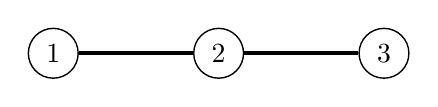
\begin{tikzpicture}[scale = .7]
\SetGraphUnit{3}
\GraphInit[vstyle=Normal]
%\renewcommand{\VertexInnerSep}{1pt}
\Vertices{line}{1,2,3}
\SetUpEdge[lw=1.5pt]
\Edges(1,2,3)
\end{tikzpicture}
\end{center}
\end{figure}
\noindent The transition matrix for a random walk on this graph is
$$
\begin{pmatrix}
0 & 1 & 0 \\
\frac12 & 0 & \frac12 \\
0 & 1 & 0
\end{pmatrix}
$$
which has stationary distribution $\left( \frac14 , \frac12 , \frac14 \right)$.
\end{proof}

\begin{prob3}
People enter the back of a queue according to a rate $\lambda$ Poisson process.  Once at the front of the queue, they take time Exp$(\mu)$ to be served and then leave the queue.  Let $X(t)$ be the number of people in the queue.\\
(a) $X(t)$ is a Markov chain.  Why is it important that the service times have exponential distribution?\\
(b) Find the generator of $X(t)$.\\
(c) For which values of $\mu, \lambda$ does the stationary distribution exist?  When it exists, find the distribution.
\end{prob3}

\begin{proof}
We will first show that, for $X(t)$ to be a Markov chain, the time it takes for a person to be served \emph{must} be exponentially distributed.  Suppose that $X(t)$ is a Markov chain.  Let $T_t$ be the total time it takes for the person at the front of the queue at time $t$ to be served.  Let $N(r,s)$ be the number of people who enter the back of the queue during the interval $(r,s)$.  Note that $T_t$ and $N(r,s)$ are independent for any values of $r,s$ and $t$.  Let $a,b$, and $c$ be any times such that $a < b < c$.

Because $X(t)$ is a Markov chain, we know that
$$\p[X(t) = x \ \forall t \in (a,c) \given X(t) = x \ \forall t \in (a,b)] = \p[X(t) = x \ \forall t \in (b,c)].$$  The lefthand side of this equality is the probability that
\begin{itemize}
\item the person at the front of the queue at time $a$ takes longer than time $c-a$ to depart, and
\item no one enters the back of the queue during the interval $(a,c)$.
\end{itemize}
given that
\begin{itemize}
\item the person at the front of the queue at time $b$ has already been there for at least a time of $b-a$, and
\item no one entered the back of the queue during the interval $(a,b)$
\end{itemize}
The righthand side is the probability that \begin{itemize}
\item the person at the front of the queue at time $b$ takes longer than time $c-b$ to depart, and
\item no one enters the back of the queue during the interval $(b,c)$
\end{itemize}
regardless of the past.  Therefore, this statement is equivalent to
$$
\p[T_a > c-a, \ N(a,c) = 0 \given T_b > b-a, \ N(a,b) = 0] = \p[T_b > c-b, \ N(b,c) = 0]
$$
This implies the following:
\begin{align}
& \ \p[T_a > c-a \given T_a > b-a] \ \p[N(b,c) = 0]
\\
= & \ \p[T_a > c-a \given T_a > b-a] \ \p[N(a,c) = 0 \given  N(a,b) = 0]
\\
= & \ \p[T_a > c-a, \ N(a,c) = 0 \given T_a > b-a, \ N(a,b) = 0]
\\
= & \ \p[T_b > c-b, \ N(b,c) = 0]
\\
= & \ \p[T_b > c-b] \ \p[N(b,c) = 0]
\end{align}
Equations (3) and (5) are obtained by using the independence of $N$ and $T$.  Equation (4) is the result of the fact that we argued above.  Finally, cancelling the factor $\p[N(b,c) = 0]$ and using the fact that $T_a$ and $T_b$ have the same distribution gives the memorylessness property:
$$ \p[T_a > c-a \given T_a > b-a] = \p[T_b > c-b] = \p[T_a > c-b]$$
Memorylessness characterizes the exponential distribution.  Therefore, $T$ must be exponentially distributed.

The generator matrix for $X(t)$ is defined by
$$
G_{0j} =
\begin{cases}
-\lambda & j = 0 \\
\lambda  & j = 1 \\
0 & \text{else}
\end{cases}
\hspace{1.5 cm}
G_{ij} = 
\begin{cases}
\mu & j = i-1 \\
-(\lambda + \mu) & j = i \\
\lambda & j = i+1 \\
0 & \text{else}
\end{cases}
$$
for $i > 0$.

Intuitively, the stationary distribution $\pi$ should exist if and only if $\lambda < \mu$.  We can solve for $\pi$ by solving the equation $\pi G = 0$.  This gives the system
$$
\begin{cases}
-\lambda \pi_0 + \mu \pi_1 = 0 \\
\lambda \pi_{i-1} - (\lambda + \mu) \pi_i + \mu \pi_{i+1}, & i > 0
\end{cases}
$$
We will show by induction that $$\pi_n = \left(\frac{\lambda}{\mu} \right)^n \pi_0$$ for all $n \geq 0$.  This is clear for $n=0$.  To show this for $n=1$, simply add $\lambda \pi_0$ to both sides of the first equation then divide both sides by $\lambda$.

Now, assume the formula holds for all $k \leq n+1$ for some $n \geq 0$.  Then the second equation gives
$$
0 = \lambda \pi_n - (\lambda + \mu)\pi_{n+1} + \mu \pi_{n+2} = \lambda \left(\frac{\lambda}{\mu}\right)^n - \left(\lambda + \mu\right) \left(\frac{\lambda}{\mu}\right)^{n+1} + \mu \left(\frac{\lambda}{\mu}\right)^{n+2}
$$
$$
\implies \pi_{n+2} = \left(\frac{\lambda}{\mu}\right)\left(\frac{\lambda}{\mu}\right)^{n+1} +\left(\frac{\mu}{\mu}\right) \left(\frac{\lambda}{\mu}\right)^{n+1} - \left(\frac{\lambda}{\mu}\right)\left(\frac{\lambda}{\mu}\right)^{n} = \left(\frac{\lambda}{\mu}\right)^{n+2}.
$$
Therefore, the stationary distribution satisfies $\pi_n = (\frac{\lambda}{\mu})^n \pi_0$ for all $n \geq 0$.

To solve for $\pi_0$, note that
$$
\sum\limits_{n=0}^\infty \left(\frac{\lambda}{\mu} \right)^n \pi_0 = \frac{\pi_0}{1-\frac{\lambda}{\mu}} = 1 \implies \pi_0 = 1 - \frac{\lambda}{\mu}.
$$
Therefore,
$$
\pi_n = \left(\frac{\lambda}{\mu} \right)^n \left(1 - \frac{\lambda}{\mu} \right)
$$
which means that the stationary distribution is geometric with parameter $1 - \frac{\lambda}{\mu}$.
\end{proof}

\begin{prob4}
Let $X(t)$ be a Markov chain on $\{1,2,3,4,5,6\}$ as follows.  When the Markov chain is in state $i$, it waits for time Exp$(i)$ and then moves to state $j$ (possibly the same), chosen by rolling a standard 6-sided die.  What is the generator of $X(t)$?  What is its stationary distribution?
\end{prob4}

\begin{proof}
The generator of $X(t)$ is given by
$$
G_{ij} =
\begin{cases}
\dfrac{i}{6} & i \neq j \\
-\dfrac{5i}{6} & i = j
\end{cases}.
$$

To solve for the stationary distribution, try to solve the detailed balance equations to check if the chain is reversible:
$$
\pi_i G_{ij} = \pi_j G_{ji} \implies
\frac{i}{6} \pi_i = \frac{j}{6}\pi_j \implies
\pi_i = \frac{j}{i} \pi_j \implies
\pi_i = \frac{\pi_1}{i}
$$
where the final equation is found inductively.  Thus,
$$
\sum\limits_{i=1}^6 \frac{\pi_1}{i} = \pi_1 \sum\limits_{i=1}^6 \frac1i = 1 \implies
\pi_1 = \frac{20}{49}
$$
$$
\implies \pi_i = \frac{20}{49i}.
$$
%To solve for the stationary distribution, we can express the equation $\pi G = 0$ as the system of inner products
%$$
%\pi \cdot G_j = \sum\limits_{i=1}^6 \frac{i\pi_1}{6} - \frac{j \pi_j}{6} - \frac{5j \pi_j}{6}
%= \frac16 \sum\limits_{i=1}^6 i\pi_i - j\pi_j = 0
%$$
%$$
%\implies \pi_j =  \frac{1}{6j} \sum\limits_{i = 1}^6 i \pi_i 
%$$

\end{proof}

\end{document}



















